%%%%%%%%%%%%%%%%%%%%%%%%%%%%%%%%%%%%%%%%%
% University/School Laboratory Report
% LaTeX Template
% Version 3.1 (25/3/14)
%
% This template has been downloaded from:
% http://www.LaTeXTemplates.com
%
% Original author:
% Linux and Unix Users Group at Virginia Tech Wiki 
% (https://vtluug.org/wiki/Example_LaTeX_chem_lab_report)
%
% License:
% CC BY-NC-SA 3.0 (http://creativecommons.org/licenses/by-nc-sa/3.0/)
%
%%%%%%%%%%%%%%%%%%%%%%%%%%%%%%%%%%%%%%%%%

%----------------------------------------------------------------------------------------
%	PACKAGES AND DOCUMENT CONFIGURATIONS
%----------------------------------------------------------------------------------------

\documentclass{article}

\usepackage[final]{pdfpages}
\usepackage{hyperref}
\usepackage{graphicx} % Required for the inclusion of images
\usepackage{natbib} % Required to change bibliography style to APA
\usepackage{amsmath} % Required for some math elements 

\setlength\parindent{0pt} % Removes all indentation from paragraphs

\renewcommand{\labelenumi}{\alph{enumi}.} % Make numbering in the enumerate environment by letter rather than number (e.g. section 6)

%\usepackage{times} % Uncomment to use the Times New Roman font

%----------------------------------------------------------------------------------------
%	DOCUMENT INFORMATION
%----------------------------------------------------------------------------------------

\title{Development Plan Deliverables Report \\ ECE 5770 \\ Microcomputer Interfacing} % Title

\author{Cody \textsc{Herndon}} % Author name

\date{\today} % Date for the report

\begin{document}

\maketitle % Insert the title, author and date

%----------------------------------------------------------------------------------------
%	SECTION I
%----------------------------------------------------------------------------------------

\section*{Forward}

The Remote Rover Training System is intended to be a lightweight, inexpensive training platform for scientists and engineers to experiment with various aspects of real-time operating systems, and system implementation and integration.  From hereon in, this project will simply be referred to as ``the Rover''.

All code for this project, as well as pertinent documentation, can be found in the project's \href{http://www.github.com/Shamshel/ECE5770}{github account}.

Sections 1.1 Determine the Process Model to be Followed, 1.2 Requirements, and 1.3 Create Tests and Hardware/Software Design were all completed in earlier exercises which were submitted to canvas throughout the semester.  These assignments may be referred to throughout the document, particularly in section 1.5 and section 1.10 where software implementation and full system testing are to take place.

%----------------------------------------------------------------------------------------
%	SECTION 2
%----------------------------------------------------------------------------------------

\section*{1.4 Review Hardware}

This exercise was completed in class as a peer review was conducted between my classmates and I.

%----------------------------------------------------------------------------------------
%	SECTION 3
%----------------------------------------------------------------------------------------

\section*{1.5 Implement/Test Hardware}

Hardware was constructed using the Tiva-C development kit\cite{Tiva-C}, ESP8266 WiFi board\cite{ESP8266}, and the NEO-6 GPS module\cite{neo-6}.

Further discussion of the construction of the hardware is discussed in Section 1.7, Implement Software, as the hardware interconnection was rather simple, the hardware implementation was driven by the software's development.

\subsection*{1. Hardware subsections}
The hardware implementation was divided into 5 major subsections:
\begin{enumerate}
  \item Tiva-C
  \item ESP8266
  \item Chassis
  \item Power Supply
  \item NEO-6

\end{enumerate}

\subsection*{2. Test each subsection and record results}

Each subsection of the hardware was implemented and then tested with software as described in Section 1.7.

\subsection*{3. Fix any flaws that you uncover}

Each subsection of the hardware did not require any major revisions.

\subsection*{4. Redraw your corrected Schematics}

Minor revisions to the schematic are outlined in the following figures.

\clearpage

\begin{figure}
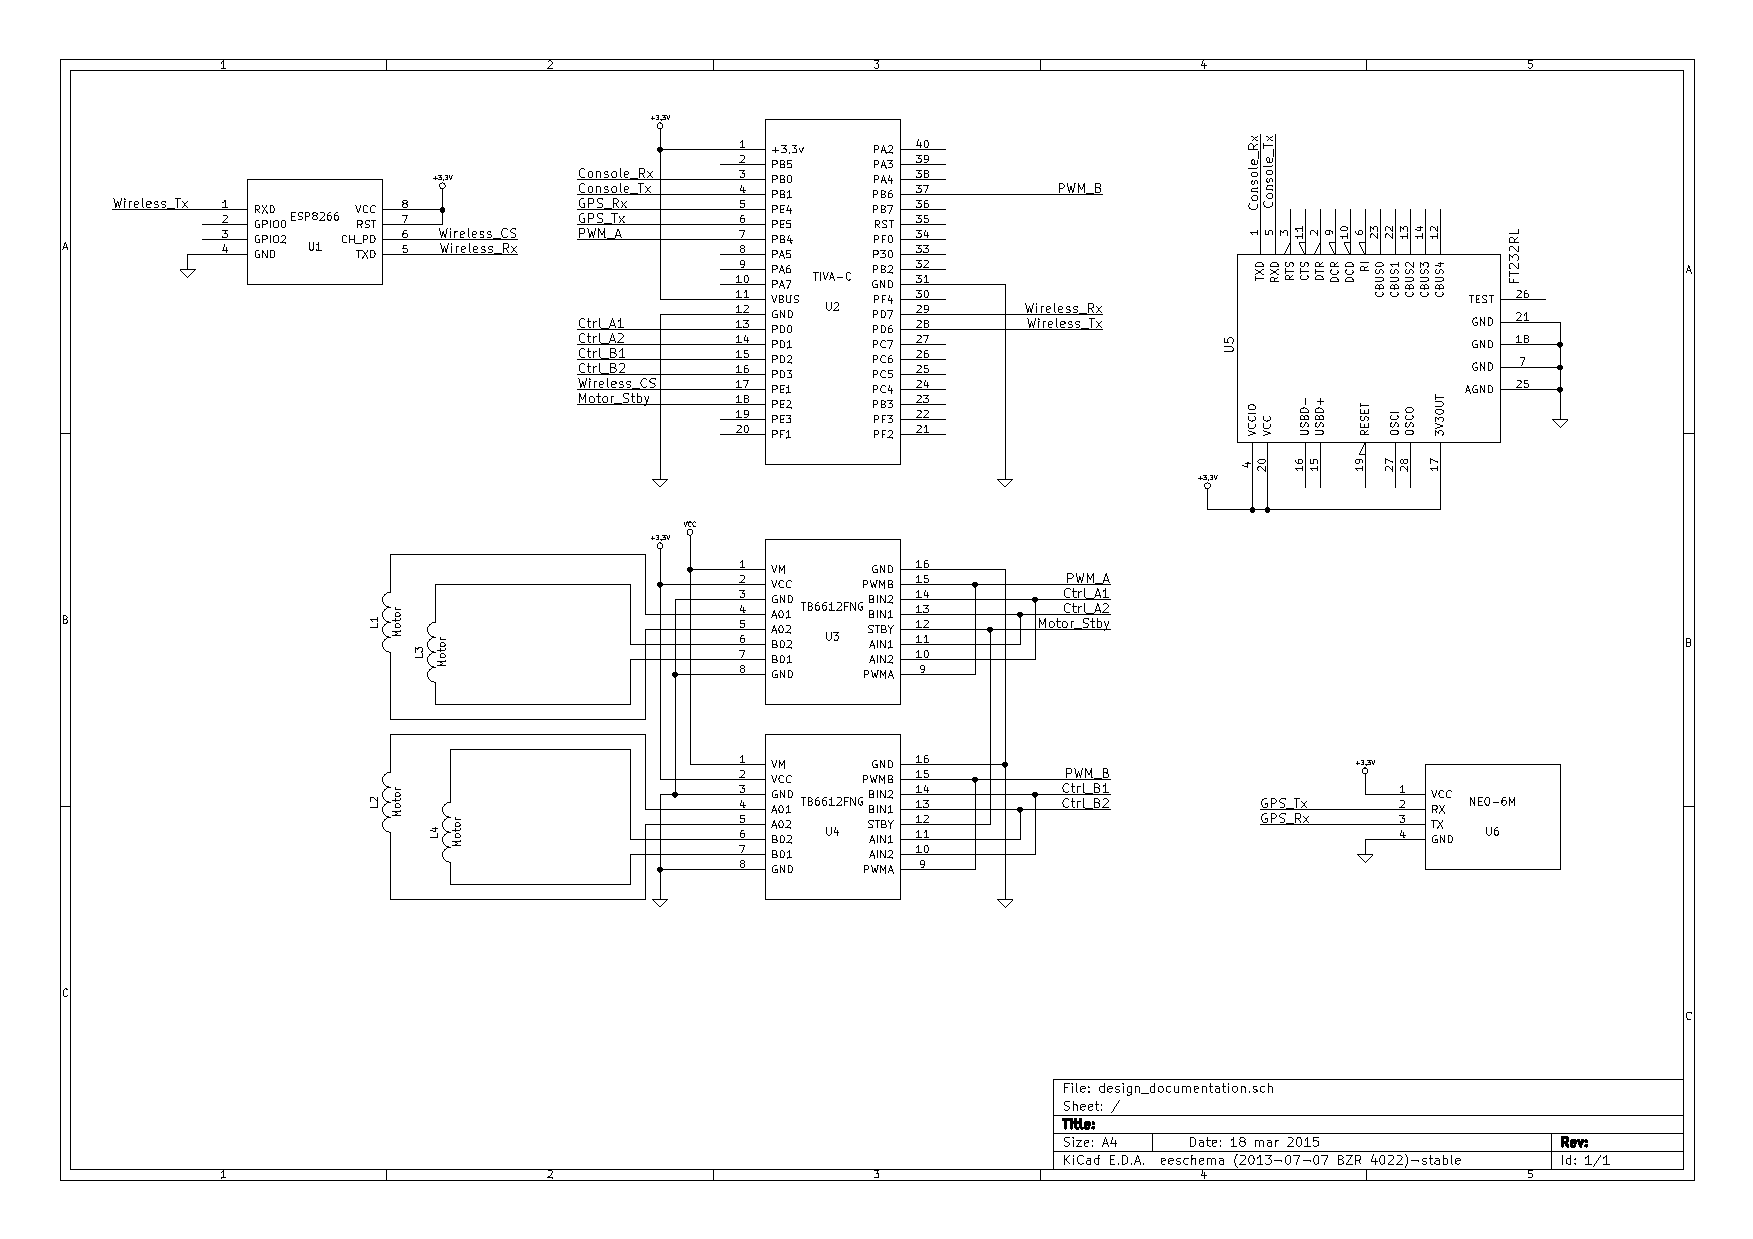
\includepdf[pages=1]{schematic}

\end{figure}
Figure 1: Initial schematic draft

\clearpage

\begin{figure}
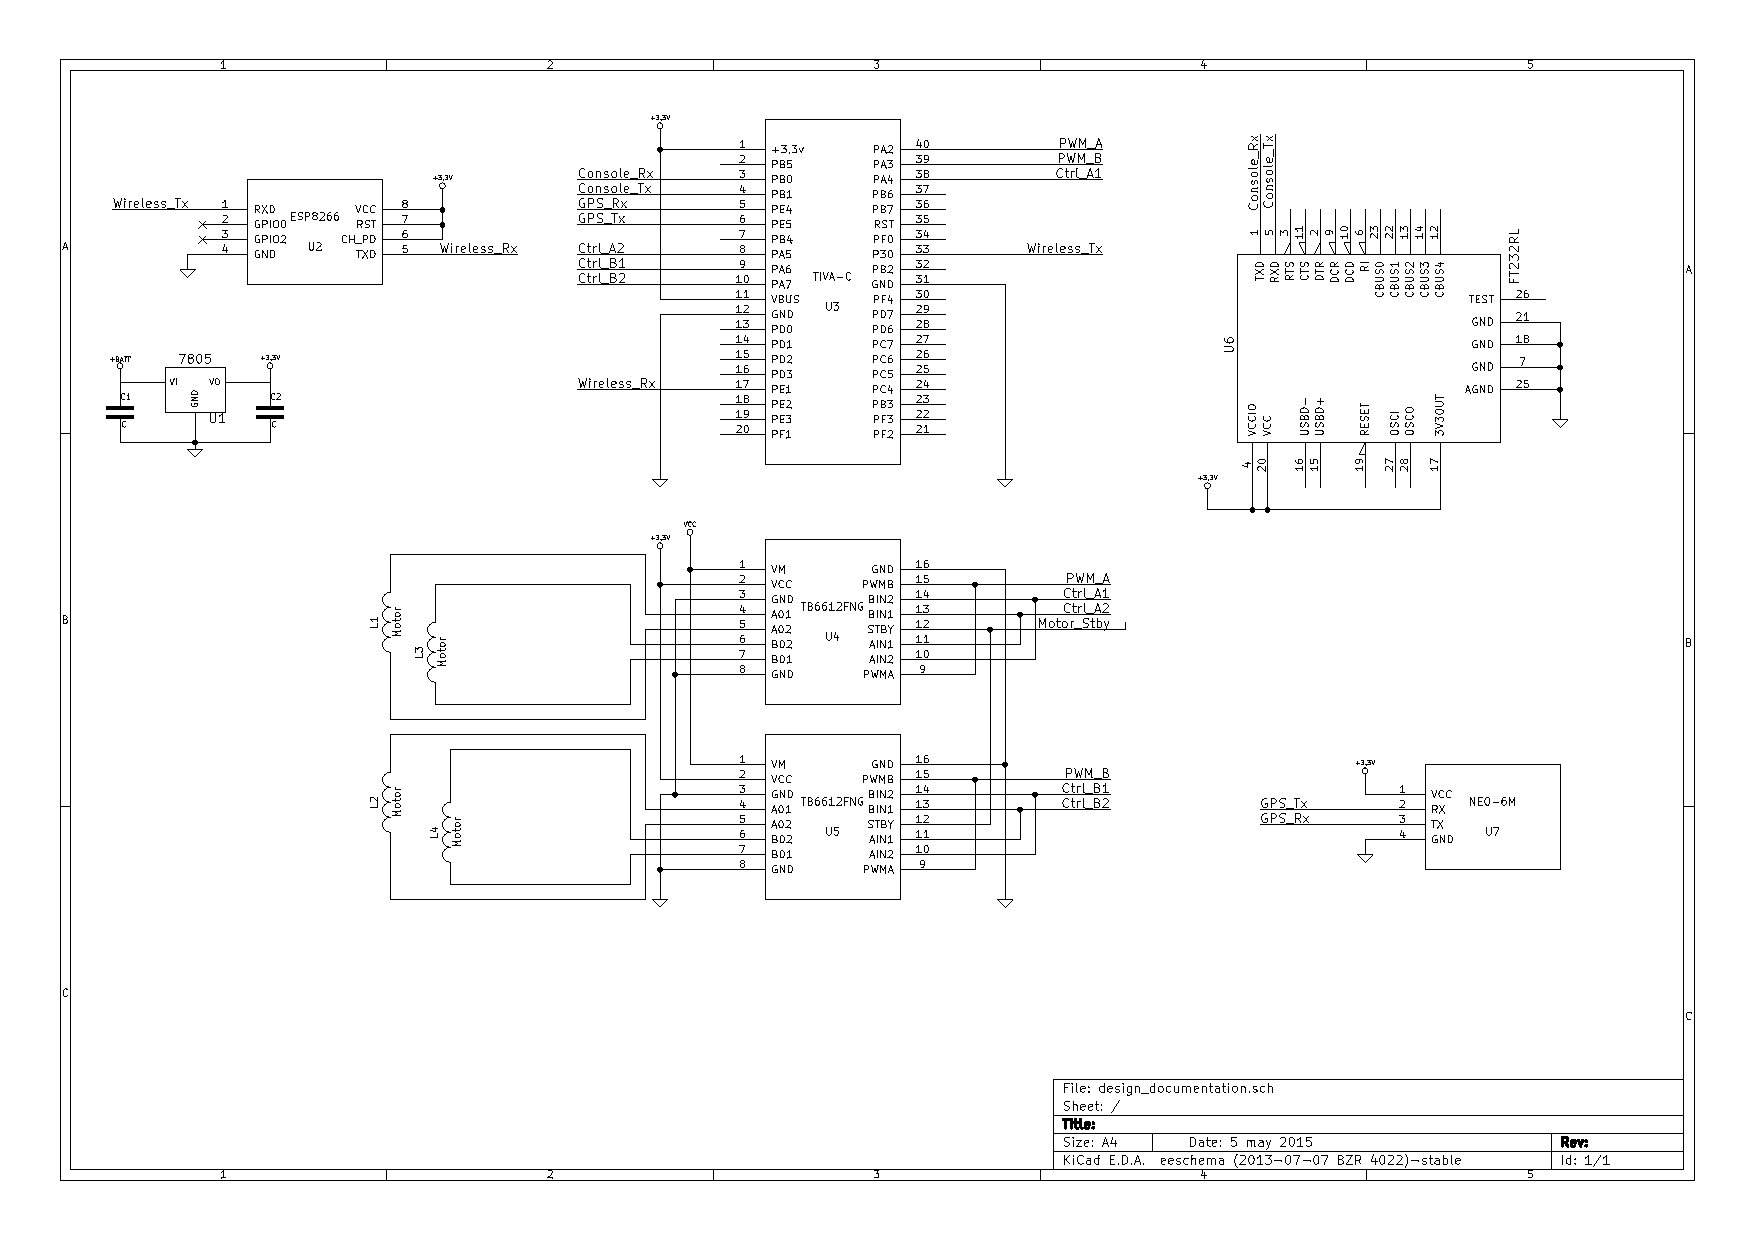
\includepdf[pages=1]{schematic_update}

\end{figure}
Figure 2: Revised schematic draft.

\clearpage

\subsection*{5. Measure Powers}
\begin{tabular}{|c|c|}
  \hline
  State & Power Consumption (W)\\\hline\hline
  Start-up & 0.375 \\\hline
  Idle &  0.3 \\\hline
  Motion & 7.2 \\\hline

\end{tabular}

%----------------------------------------------------------------------------------------
%	SECTION 4
%----------------------------------------------------------------------------------------

\section*{1.6 Review Software Design}

\subsection*{1. Review your software design with a classmate.}

This exercise was done in class.  The classmate found the design to be satisfactory.

\subsection*{2.  Make any adjustments as necessary.}

No major adjustments were made during the course of this software design review.

%----------------------------------------------------------------------------------------
%	SECTION 5
%----------------------------------------------------------------------------------------

\section*{1.7 Implement Software}

\subsection*{Cycle 1}

Cycle 1 focused on implementing the core kernel code and the core system architecture for the Micro-Kernel real-time system.

\subsubsection*{Design}
The system design for the core kernel was that of a Micro kernel\cite{microkernel}.  The micro kernel architecture was selected due to its inherit simplicity and compactness.  It was entirely possible that this software system could be pushing the limits of the Tiva-C's code size and computational speed limits, so a high-speed micro kernel was selected for the core.  The Real-time scheduling portion of the system was designed to be far more complicated than the final implementation, but the system was finally implemented using a simple RM or RR schedule with tasks being registered upon the initialization of the system.

\subsubsection*{Develop}
Development of the kernel was implemented using strict c, as was the remainder of the software, using the Modular Programming in C\cite{modular-c} tutorial as a guide.  Final implementation can be found at \href{https://github.com/Shamshel/ECE5770/commit/c00127be4eaf347272067aba7e434a1e986104e6}{the github site}.

\subsubsection*{Test}
The kernel was implemented in such a manner as to be tested on an x86 desktop, and thus is as platform agnostic as possible.  The program can be made on any platform with the required dependencies, namely the cunit test suite and gcc.  Unit testing confirmed the functionality of the system.

\subsection*{Cycle 2}

Cycle 2 focused on porting the kernel to the Tiva-C development board and is thus implemented using TI's development software and the \emph{arm-none-eabi-gcc} compiler.  This cycle completed with the successful execution of the kernel code on the Tiva-C board.

\subsubsection*{Design}
the system design is unchanged from the previous cycle, but uses an LED blink function embedded in the kernel code to indicate successful code execution.  Further confirmation was performed with the \emph{arm-none-eabi-gdb} program.

\subsubsection*{Develop}
Porting the system was completed relatively quickly.  The biggest dilemma in this system port was working with the gcc cross-compilers and makefile.  Results of the implementation for this section can be found in \href{https://github.com/Shamshel/ECE5770/commit/7a165da5f1471905e4bebfb925ed24c03c95f8b4}{the github site}.

\subsubsection*{Test}
The system was implemented to run on the Tiva-C board, and thus was more difficult to debug.  The system was tested and confirmed working with a hardware pin indicator, blinky LED, and gdb tracing.

\subsection*{Cycle 3}

Cycle 3 focused on implementing UART hardware drivers to communicate with the workstation computer to ensure easier debugging, and later interface to the WiFi and GPS peripherals.

\subsubsection*{Design}
The implementation of the UART driver was completed in a similar manner to the implementation of the functions used to debug the kernel.  UART driver API for the Tiva-C was described in the documentation accompanying the software libraries for the device\cite{SW-TM4C}.

\subsubsection*{Develop}
Development proceeded smoothly, as the API given in \cite{SW-TM4C} was clear and concise.  This development cycle completed with the successful echo of the debug input from the PC to the Tiva-C and back to the PC. The results of the development process can be found in \href{https://github.com/Shamshel/ECE5770/commit/0b449546cf80b91c1b842a0b21c7e088970f24e6}{the github account}.

\subsubsection*{Test}
Testing for this cycle concluded when the UART could successfully and easily echo input from the console out to the computer without dropping characters or requiring represses.

\subsection*{Cycle 4}

Cycle 4 focused on implementing the WiFi driver and controller functionality.  The WiFi driver functionality was to detect a reception of a newline and forward the results to the controller, thus abstracting the driver implementation away from the controller.  The controller was to then implement a simple state machine, detect certain keywords to trigger a state change, and send corresponding responses to the WiFi module and main controller or motor controller.

\subsubsection*{Design}
The controllers and drivers implemented here were intended to be modeled on the dummy function from Cycle 1.  The drivers were implemented in this fashion to avoid a deadlock or starvation of the other tasks.

\subsubsection*{Develop}
Development proceeded with some hitches.  The Kernel needed increased capabilities in order to facilitate string parsing for the state machine to function properly.  The system is otherwise largely unchanged.  The results of this development cycle can be see in the \href{https://github.com/Shamshel/ECE5770/commit/b789e506165f0ada4f6a83999845b9865b585fe4}{github account}.

\subsubsection*{Test}
Testing for this cycle concluded when the system was capable of communicating with the ESP8266 and parsing commands from its interface.

\subsection*{Cycle 5}
Cycle 5 focused on implementing the motor drivers to enable movement with the Multi-Chassis kit\cite{multi-chassis}.  The Power and chassis hardware subsystems were implemented here.

\subsubsection*{Design}
Design again focused on the simple task developed for Cycle 1.  The motor driver receives messages from the WiFi controller and then commands the Chassis subsystem to move based on commands received from the ESP8266.

\subsubsection*{Develop}
Development went smoothly for this cycle, as the motor driver turned out to be comparatively simple to implement.  See \href{https://github.com/Shamshel/ECE5770/commit/7c3a11e5c96f9c3f0fa2e360a50f103b7e07cb66}{the github} for the result of the implementation.

\subsubsection*{Test}
Testing concluded when the Motor driver was able to take commands from the WiFi controller and translate those commands successfully into motion on the Multi-Chassis kit.

%----------------------------------------------------------------------------------------
%	SECTION 6
%----------------------------------------------------------------------------------------

\section*{1.8 Review Software Implementation}

\subsection*{1. Review your software with a classmate.}
Software was reviewed at the conclusion of each cycle with the members of the group who were not responsible for the development of software.

\subsection*{2. Make any adjustments necessary.}
One patch was required for the WiFi controller system as outlined in \href{https://github.com/Shamshel/ECE5770/commit/7c3a11e5c96f9c3f0fa2e360a50f103b7e07cb66}{the github} following Cycle 5.

%----------------------------------------------------------------------------------------
%	SECTION 7
%----------------------------------------------------------------------------------------

\section*{1.9 Test Implementations of Software Modules}
Various implementations of the software were tested and debugged during the development cycles outlined above.  Refer to \href{https://github.com/Shamshel/ECE5770}{the github} for patch notes and development notes.

%----------------------------------------------------------------------------------------
%	SECTION 8
%----------------------------------------------------------------------------------------

\section*{1.10 Test Full System to Requirements}
Some tests were not able to be performed, as the system was not completed to the full specifications outlined in the Customer Requirements Documents.  Thus, the following table outlines the successes and failures of the system to date.

\begin{tabular}{|c|c|p{8cm}|c|}
  \hline
  Item & Requirement & Test & Met\\\hline
  2.1 & 50 lbs weight limit & Place the rover on a scale such that all its weight is supported on the scale.  The scale should report no more than 50 lbs. & Y \\\hline
  2.2 & dimension limits & Measure 3 feet in each dimension, the System should not project beyond the measurements in that dimension. & Y \\\hline
  2.3 & accessibility requirements & Observe that if the System encloses its electronics that the electrical system can be accessed through a single access panel & Y \\\hline
  2.4 & drive requirements & Command the System to travel forward 10 ft on carpet of 1/2 inch thickness. & Y \\\hline
  3.1.1 & battery capacity & Observe that the manufacturer rates the installed battery at the required capacity. & Y \\\hline
  3.1.2 & battery rechargeability & Observe that the manufacturer denotes that the installed battery can be recharged. & N \\\hline
  3.1.3 & idle endurance & Activate the System and observe that it is capable of operating for at least one hour. & Y \\\hline
  3.1.4 & active endurance & Activate the System and transmit a command to traverse forward.  Observe that the System is capable of continuing to travel for 10 minutes. & Y \\\hline
  3.2.1 & remote control & Observe that the System is capable of receiving commands and sending data without being physically connected to the base station. & Y \\\hline
  3.2.2 & additional hardware & Observe that the base station is not attached to hardware that is not commercial off the shelf to communicate with the System. & Y \\\hline
  3.2.3 & command range & Place the System 50 feet from the base station. Send a command from the base station to the System, observe that the System responds. & Y \\\hline
  3.2.4 & response range & Place the System 50 feet from the base station. Observe that the System responds. & Y \\\hline
  3.2.5 & update range & Place the System 50 feet from the base station. Attempt to update the System's software.  Observe that the System is properly updated. & N \\\hline
  3.3.1 & estimation accuracy & Activate the System and command it to travel forward 10 ft.  Observe that the recorded distance is within 1 ft of the distance traveled. & N \\\hline

\end{tabular}

\begin{tabular}{|c|c|p{8cm}|c|}
  \hline
  3.3.2 & battery power & Activate the System.  Observe that the system reports an estimate of remaining battery power to within 10\% of the manufacturer provided model of the battery's power. & N \\\hline
  3.3.3 & motor power & Place the System in such a way as the motion system is able to travel freely.  Activate the System and command it to travel forward.  Observe that the power dissipated by the motors as measured by a test equipment is within 10\% of the dissipation reported by the System. & N \\\hline
  4.1.1 & speed limit & Activate the System on a flat, smooth surface and command it to travel forward 10 seconds.  Measure the distance traveled and ensure that the system travels at no more than 3 mph. & Y \\\hline
  4.1.2 & rotation speed & Activate the System on a flat, smooth surface and command it to rotate 360 degrees.  Record the amount of time required to rotate, ensure that it is no less than 6 degrees per second. & Y \\\hline

\end{tabular}

\section*{Conclusion}
The final system developed is very nearly the system described in the proposal document.  Unfortunately, time and resource constraints have caused the project to fall behind schedule.  A few more development cycles to fully implement the GPS controller and extend the functionality of the WiFi controller to be able to POST data to a website would have fulfilled all the outlined requirements.  Furthermore, a simple change in battery source from 1.5v AA batteries to a rechargeable Li-Ion or NICD battery pack would have fulfilled requirement 3.1.2.

A final demonstration of the system in action can be found on \href{https://www.youtube.com/watch?v=gsIGP2L7iuk}{YouTube}.

%----------------------------------------------------------------------------------------
%	BIBLIOGRAPHY
%----------------------------------------------------------------------------------------

\bibliographystyle{plain}
\bibliography{sample}

%----------------------------------------------------------------------------------------


\end{document}
